\documentclass[12pt,twoside]{article}
\usepackage{amsmath, amssymb}
\usepackage{amsmath}
\usepackage[active]{srcltx}
\usepackage{amssymb}
\usepackage{amscd}
\usepackage{makeidx}
\usepackage{float}
\usepackage{amsthm}
\usepackage{algpseudocode}
\usepackage{algorithm}
\usepackage{graphicx}
\usepackage[spanish, es-tabla]{babel}
\usepackage{multirow}
\usepackage{cite}
\renewcommand{\baselinestretch}{1}
\graphicspath{{images/}}
\setcounter{page}{1}
\setlength{\textheight}{21.6cm}
\setlength{\textwidth}{14cm}
\setlength{\oddsidemargin}{1cm}
\setlength{\evensidemargin}{1cm}
\pagestyle{myheadings}
\thispagestyle{empty}
\markboth{\small{Pr\'actica 7. Alan, Josu\'e}}{\small{.}}
\date{}
\begin{document}
\centerline{\bf An\'alisis de Algoritmos, Sem: 2020-1, 3CV2, Pr\'actica 6, 2 de octubre}
\centerline{}
\centerline{}
\begin{center}
\Large{\textsc{Pr\'actica 7: Algoritmo de Strassen}}
\end{center}
\centerline{\bf{Alan Romero Lucero, Josu\'e David Hern\'andez Ram\'irez}}
\centerline{}
\centerline{Escuela Superior de C\'omputo}
\centerline{Instituto Polit\'ecnico Nacional, M\'exico}
\centerline{$alanrl.escom@gmail.com, josuehernandezr082@gmail.com$}
\newtheorem{Theorem}{\quad Theorem}[section]
\newtheorem{Definition}[Theorem]{\quad Definition}
\newtheorem{Corollary}[Theorem]{\quad Corollary}
\newtheorem{Lemma}[Theorem]{\quad Lemma}
\newtheorem{Example}[Theorem]{\quad Example}
\bigskip
\textbf{Resumen:} Para la multiplicaci\'on de matrices se implementara el algoritmo de Strassen, y mediante gr\'aficas se mostrar\'a su complejidad. Adem\'as ser\'a comparado con el algoritmo de multiplicaci\'on usual.{\bf Palabras Clave:} {\textit{divide y vencer\'as, matrices, producto matricial,Strassen}}
\section{Introducci\'on}

La multiplicaci\'on de matrices resulta ser un problema algo particular, debido al algoritmo que lo soluciona. El algoritmo que lo soluciona es simple, aplicando el producto matricial simple se obtiene una complejidad $\theta(n^3)$. Entonces, intentar \textit{dividir y vencer} parece una buena opci\'on, dividiendo las matrices cuadradas en cuatro cuadrantes y haciendo un algoritmo recursivo, sin embargo, su complejidad sigue siendo $\theta(n^3)$. Por esto, se implementara el algoritmo de Strassen que presume de una complejidad de $\theta(n^2.8)$ y se comparar\'a su comportamiento con matrices muy grandes contra el algoritmo m\'as tradicional.

\section{Conceptos B\'asicos}

El problema que se resolver\'a esta planteado de la siguiente forma: Se tienen dos matrices cuadradas \textit{$A_{nxn}$} y \textit{$B_{nxn}$}, de forma tal que $k = \log_2{n}$, es decir, son matrices cuadradas de tama\~no potencia de dos. Esta limitante es importante debido al funcionamiento del algoritmo de Strassen.

\subsection{Producto usual de matrices}

El producto de matrices es una operaci\'on compleja que requiere de muchas iteraciones. Cuando se multiplica la matriz A y B, para obtener una matriz C, cada celda de C se obtiene con el producto punto de la fila de A y la columna de B correspondientes a la posici\'on de la celda de C.

\begin{figure}[H]
    \centering
    \begin{algorithmic}
        \Procedure{Producto}{$A \longleftarrow[n][n],B\longleftarrow[n][n]$}
            \State $C \longleftarrow [n][n]$
            \For{ i \textbf{from} 0 \textbf{to} n}
                \For{ j \textbf{from} 0 \textbf{to} n}
                    \For{ k \textbf{from} 0 \textbf{to} n}
                        \State $C[i][j] \longleftarrow A[i][k]*B[k][j]$
                    \EndFor
                \EndFor{}
            \EndFor
            \State \textbf{return} $C$
        \EndProcedure
    \end{algorithmic}
    \caption{Algoritmo del producto de matrices}
    \label{fig:producto}
\end{figure}

Para calcular su complejidad, por bloques, todos los \textit{\textbf{for's}} que aparecen van siempre de $0$ a $n$, por lo que su complejidad es $\theta(n) = n$. Ahora, al ser bloques \textit{\textbf{for}} se multiplican desde adentro hacia afuera la complejidad, por lo que la complejidad del algoritmo es $\theta(n^3)$.

\subsection{Algoritmo de Strassen}

El algoritmo de Strassen recupera un poco de la implementaci\'on del algoritmo recursivo, que se muestra en la Figura \ref{fig:strassen_new}. La matriz de tama\~no $n$ es divida en cuadrantes, donde cada cuadrantes es una matriz de tama\~no $\frac{n}{2}$. Esta manera de \textit{dividir y vencer} es inefectiva en el caso del algoritmo recursivo normal, dando como resultado una complejidad $\theta(n^{\log_2{8}}) = \theta(n^3)$, la misma complejidad que con el algoritmo usual debido a que la cantidad de multiplicaciones que debe hacer para obtener los cuatro cuadrantes es de ocho.
\begin{figure}[H]
    \centering
    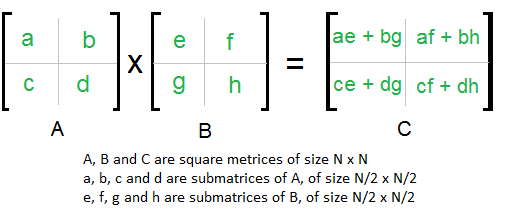
\includegraphics{strassen_new.png}
    \caption{Cuadrantes y operaciones del algoritmo recursivo convencional para el producto de matrices [1]}
    \label{fig:strassen_new}
\end{figure}

Ahora bien, el algoritmo de Strassen no realiza las mismas operaci\'on a los cuadrantes. Se aplican diversas operaciones para obtener 7 partes diferentes, que se van a operar entre s\'i para obtener cada cuadrante del resultado de la multiplicaci\'on, como se aprecia en la Figura \ref{fig:strassen_new_new}.

\begin{figure}[H]
    \centering
    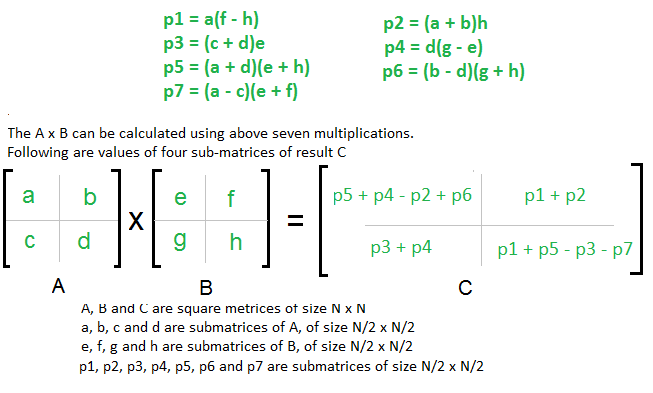
\includegraphics{stressen_formula_new_new.png}
    \caption{Formulas y operaciones aplicadas en el algoritmo de Strassen para la multiplicaci\'on de matrices [1]}
    \label{fig:strassen_new_new}
\end{figure}

Primero, hace falta tener los algoritmos para las sumas y restas de las matrices, los cuales evidentemente tienen complejidad $\theta(n^2)$. La divisi\'on de las matrices A y B en cuadrantes no requiere de ning\'un algoritmo especial ni de iteraciones, etc\'etera, por lo que su complejidad es $\theta(1)$. Finalmente se tiene que plantear la ecuaci\'on recursiva, pero antes a agrega el pseudo c\'odigo.

\begin{figure}[H]
    \centering
    \begin{algorithmic}
        \Procedure{suma/resta}{$M \longleftarrow [n][n], N \longleftarrow [n][n]$}
            \State $R \longleftarrow [n][n]$
            \For{ i \textbf{from} 0 \textbf{to} n}
                \For{ j \textbf{from} 0 \textbf{to} n}
                    $R[i][j] \longleftarrow M[i][j] \pm N[i][j]$
                \EndFor
            \EndFor
            \State \textbf{return} $R$
        \EndProcedure
    \end{algorithmic}
    \caption{Algoritmos para la suma y resta de dos matrices}
    \label{fig:sum_subs}
\end{figure}

\begin{figure}[H]
    \centering
    \begin{algorithmic}
        \Procedure{strassen}{$A\longleftarrow [n][n], B \longleftarrow [n][n]$}
            \If{$n \leq 1$}
                \State $C \longleftarrow [0][0]$
                \State $C[0][0] \longleftarrow A[0][0]*B[0][0]$
                \State \textbf{return} $C$
            \Else
                \State $C \longleftarrow [n][n]$
                \State $A_{11}, A_{12}, A_{21}, A_{22} \longleftarrow SUB_MATRICES(A)$
                \State $B_{11}, B_{12}, B_{21}, B_{22} \longleftarrow SUB_MATRICES(B)$
                \State $S1 \longleftarrow STRASSEN(SUMA(A_{11}, A_{22}), SUMA(B_{11}, B_{22}))$ // P5
                \State $S2 \longleftarrow STRASSEN(SUMA(A_{21},A_{22}), B_{11})$ // P3
                \State $S3 \longleftarrow STRASSEN(A_{11}, RESTA(B_{12}, B_{22}))$ // P1
                \State $S4 \longleftarrow STRASSEN(A_{22}, RESTA(B_{21}, B_{11}))$ // P4
                \State $S5 \longleftarrow STRASSEN(SUMA(A_{11}, A_{12}), B_{22})$ // P2
                \State $S6 \longleftarrow STRASSEN(RESTA(A_{21}, A_{11}), SUMA(B_{11}, B_{12}))$ // -P7
                \State $S7 \longleftarrow STRASSEN(RESTA(A_{12}, A_{22}), SUMA(B_{21}, B_{22}))$ // P6
                \State $C_{11},C_{12},C_{21},C_{22} \longleftarrow SUM_MATRICES(C)$
                \State $C_{11} \longleftarrow RESTA ( SUMA ( SUMA ( S1, S4 ), S7 ), S5 )$
                \State $C_{12} \longleftarrow SUMA ( S3, S5 )$
                \State $C_{21} \longleftarrow SUMA ( S2, S4 )$
                \State $C_{22} \longleftarrow SUMA ( RESTA ( S1, S2 ), SUMA ( S3, S6 ) )$
                \State \textbf{return} $MATRIZ(C_{11},C_{12},C_{21},C_{22})$
            \EndIf
        \EndProcedure
    \end{algorithmic}
    \caption{Algoritmo de Strassen}
    \label{fig:strassen}
\end{figure}

Ahora, para calcular la complejidad del algoritmo, se plantea la funci\'on $T(n)$ siendo $n$ el tama\~no del arreglo.Se realiza la operaci\'on de Strassen siete veces para obtener las siete partes que despu\'es de operan entre s\'i, adem\'as de las suma que se realizan para obtener cada cuadrante de complejidad $\theta(n) = n^2$, excepto $n \leq 1$, que es constante. La complejidad de este termina siendo de $\theta(n^{\log_2{7}}) = \theta(n^{2.8})$, que no es una gran mejora, pero es algo


\section{Experimentaci\'on y Resultados}
En las siguientes dos subsecciones se presentar\'an los resultados ontenidos a tr\'aves de la implementaci\'on de los algoritmos descritos anteriormente.
\subsection{Algoritmo de Strassen en acci\'on}
En esta subsecci\'on se muestra el funcionamiento del algoritmo de Strassen, \'unicamente funciona con matrices cuadradas. Como se puede apreciar en la siguientes figuras, el algoritmo de Strassen se compara con una función propuesta y podemos notar su comportamiento con respecto al tiempo. 
\newline \newline
Esto se puede apreciar hasta la octava en\'esima potencia, ya que, al sugerir el calculo que supere la octava potencia, se proceder\'a con la comparaci\'on del algoritmo de producto de matrices.
\begin{figure}[H]
    \centering
    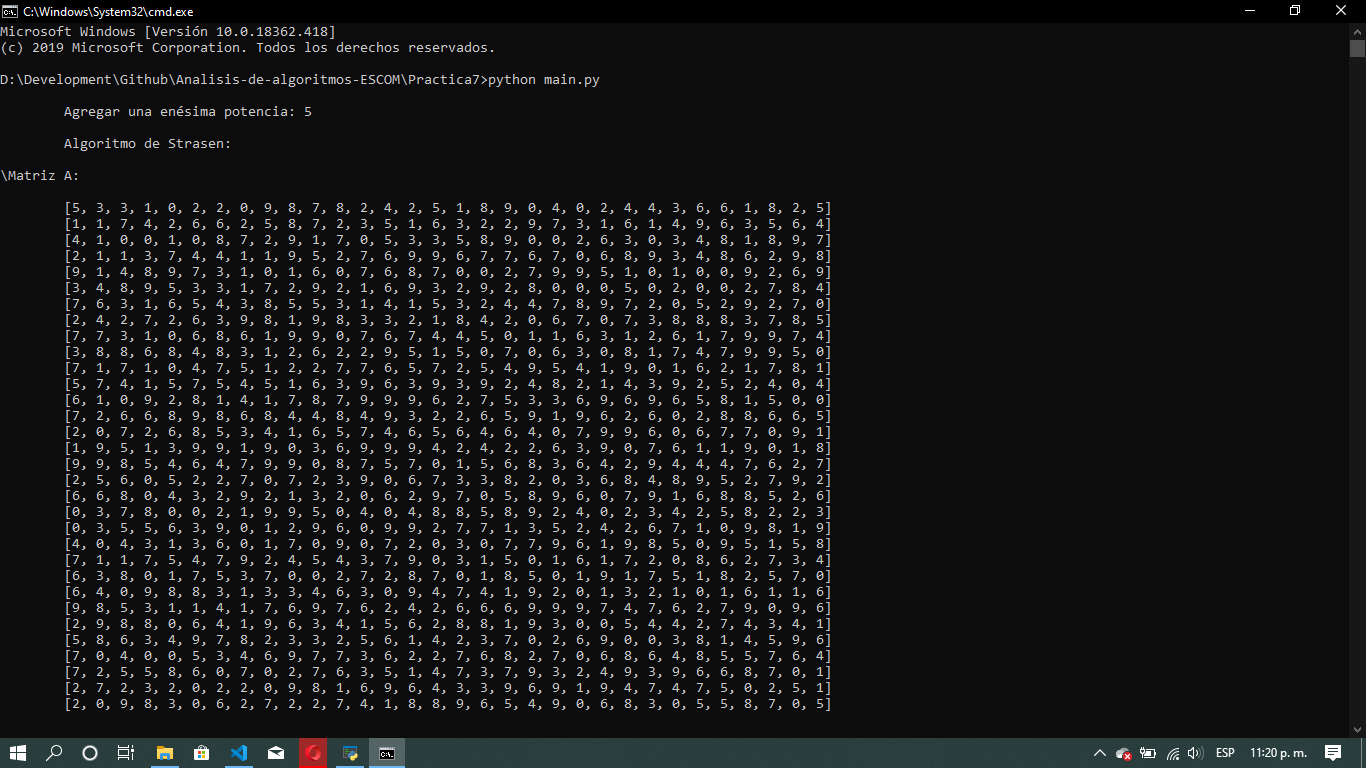
\includegraphics[scale=0.35]{strassen1.png}
    \caption{Algoritmo de Strassen en ejecuci\'on}
    \label{fig:strassen_exec}
\end{figure}
\begin{figure}[H]
    \centering
    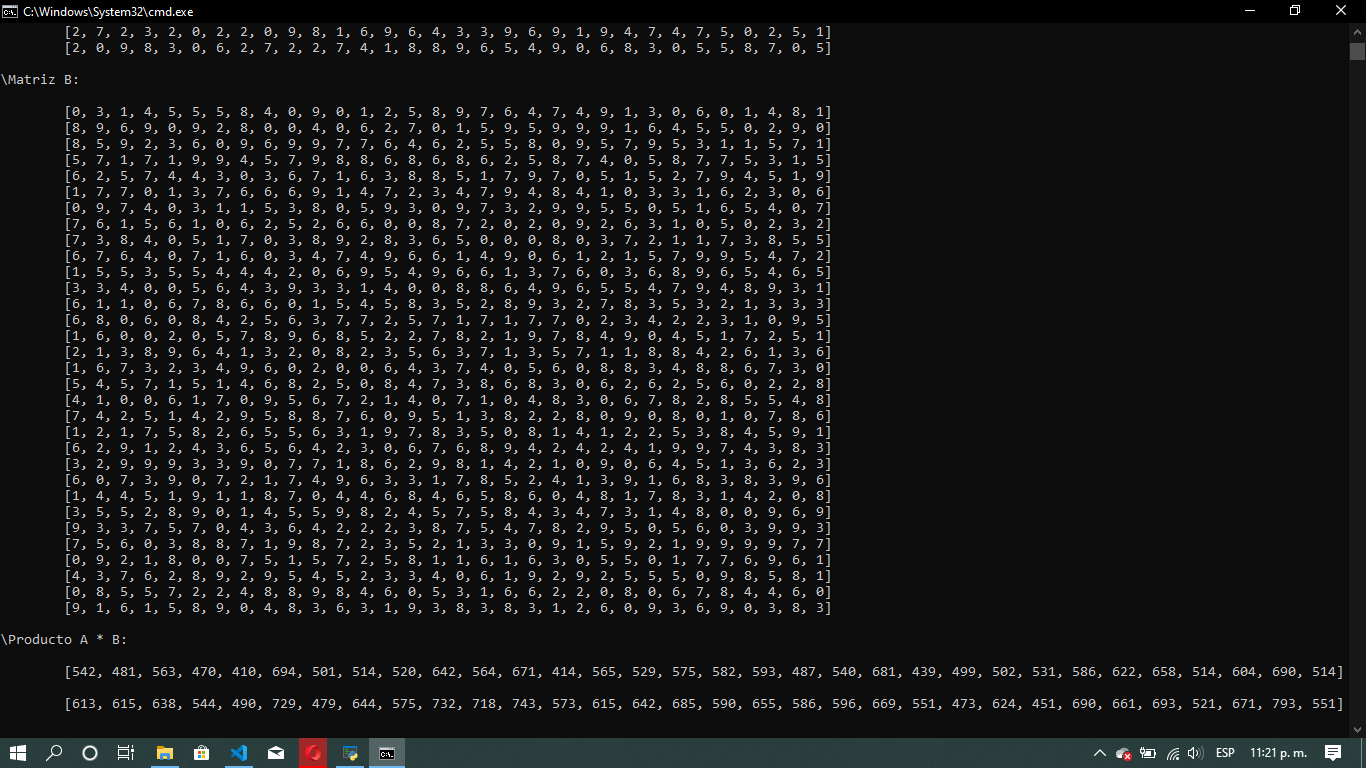
\includegraphics[scale=0.35]{strassen2.png}
    \caption{Algoritmo de Strassen en ejecuci\'on}
    \label{fig:strassen_exec}
\end{figure}
\begin{figure}[H]
    \centering
    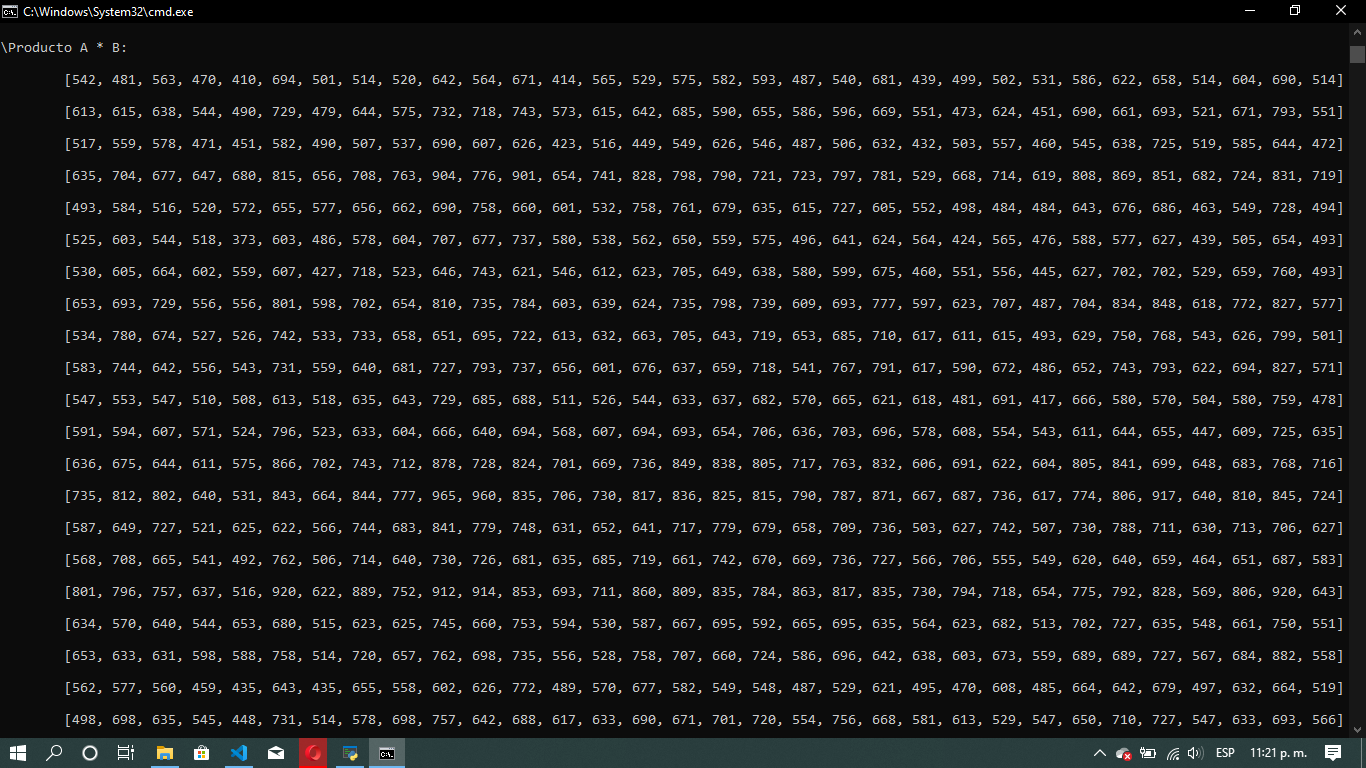
\includegraphics[scale=0.35]{strassen3.png}
    \caption{Algoritmo de Strassen en ejecuci\'on}
    \label{fig:strassen_exec}
\end{figure}
\begin{figure}[H]
    \centering
    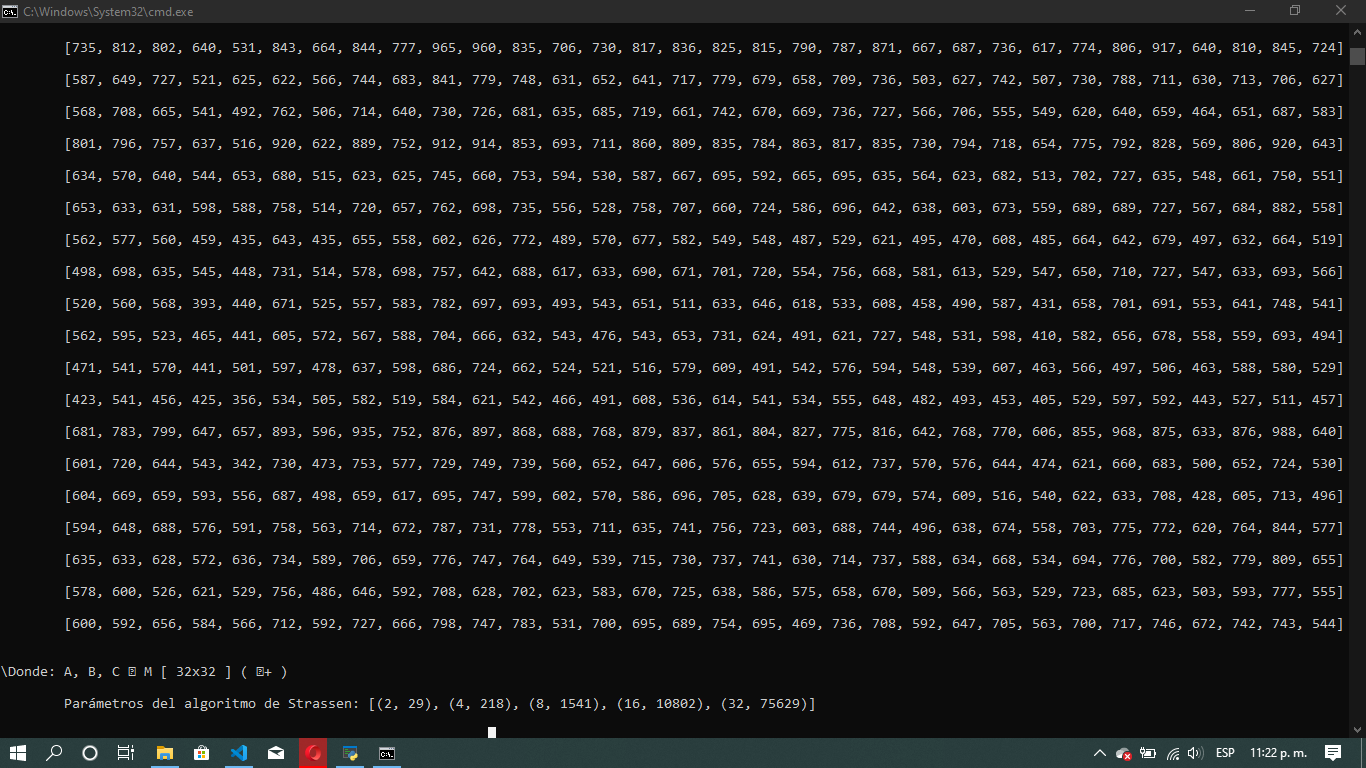
\includegraphics[scale=0.35]{strassen4.png}
    \caption{Algoritmo de Strassen en ejecuci\'on}
    \label{fig:strassen_exec}
\end{figure}
\begin{figure}[H]
    \centering
    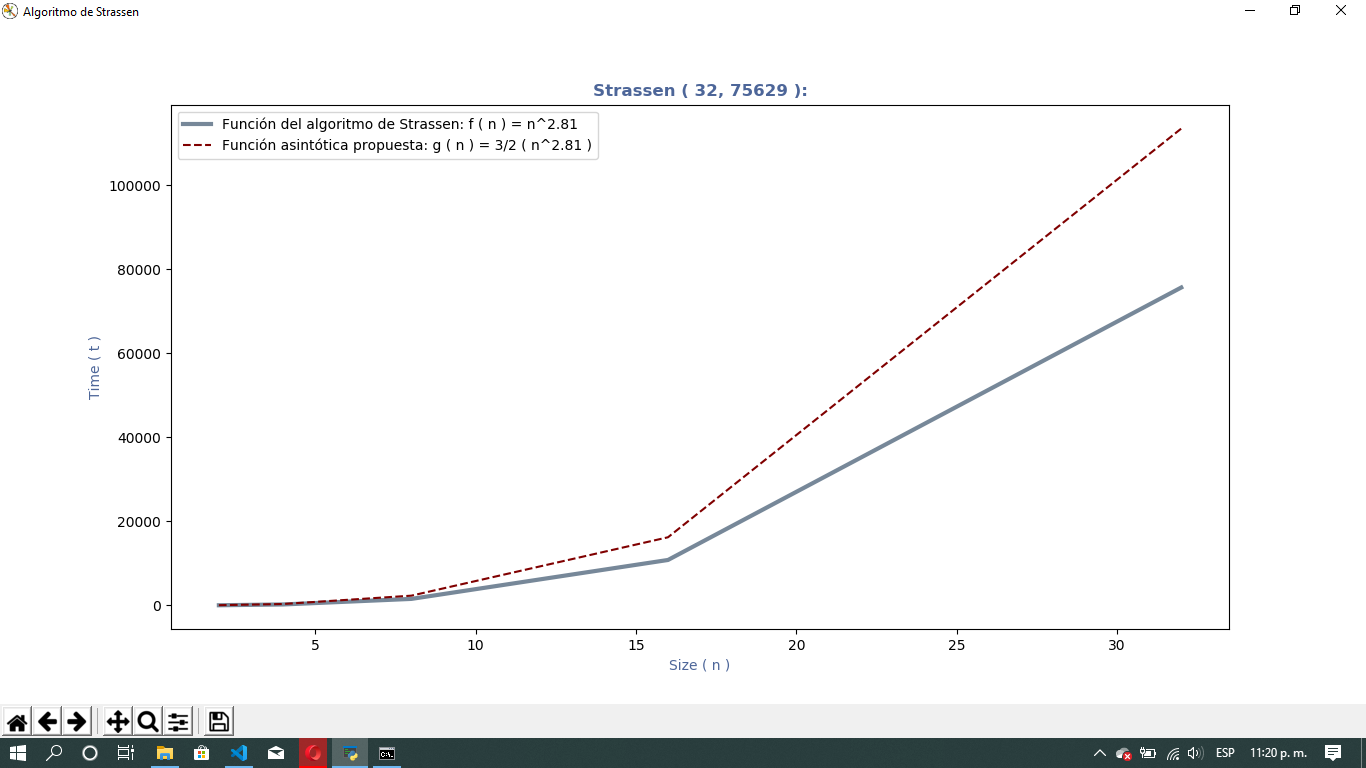
\includegraphics[scale=0.35]{strassen5.png}
    \caption{Gr\'afica del algoritmo de Strassen}
    \label{fig:strassen_graph}
\end{figure}
\subsection{Algoritmo usual vs. Strassen}
Como se describió anteriormente, para que la comparación se logre, se necesita que se introduzca una en\'esima potencia mayor o igual a 8 para que esto se ejecute.
\newline \newline
Como se ver\'a mas adelante, se ha omitido mostrar todas las matrices, puesto que se introdujo la octava potencia, por ende, son matrices cuadradas de 256 x 256, bastantes grandes y dif\'iciles de apreciar.
\newline \newline
La ultima figura de esta subsecci\'on se muestra la comparaci\'on de los algoritmos con los mismos datos, y se puede apreciar la diferencia que hay entre unas d\'ecimas de complejidad, como afecta esto al tiempo de ejecuci\'on.
\begin{figure}[H]
    \centering
    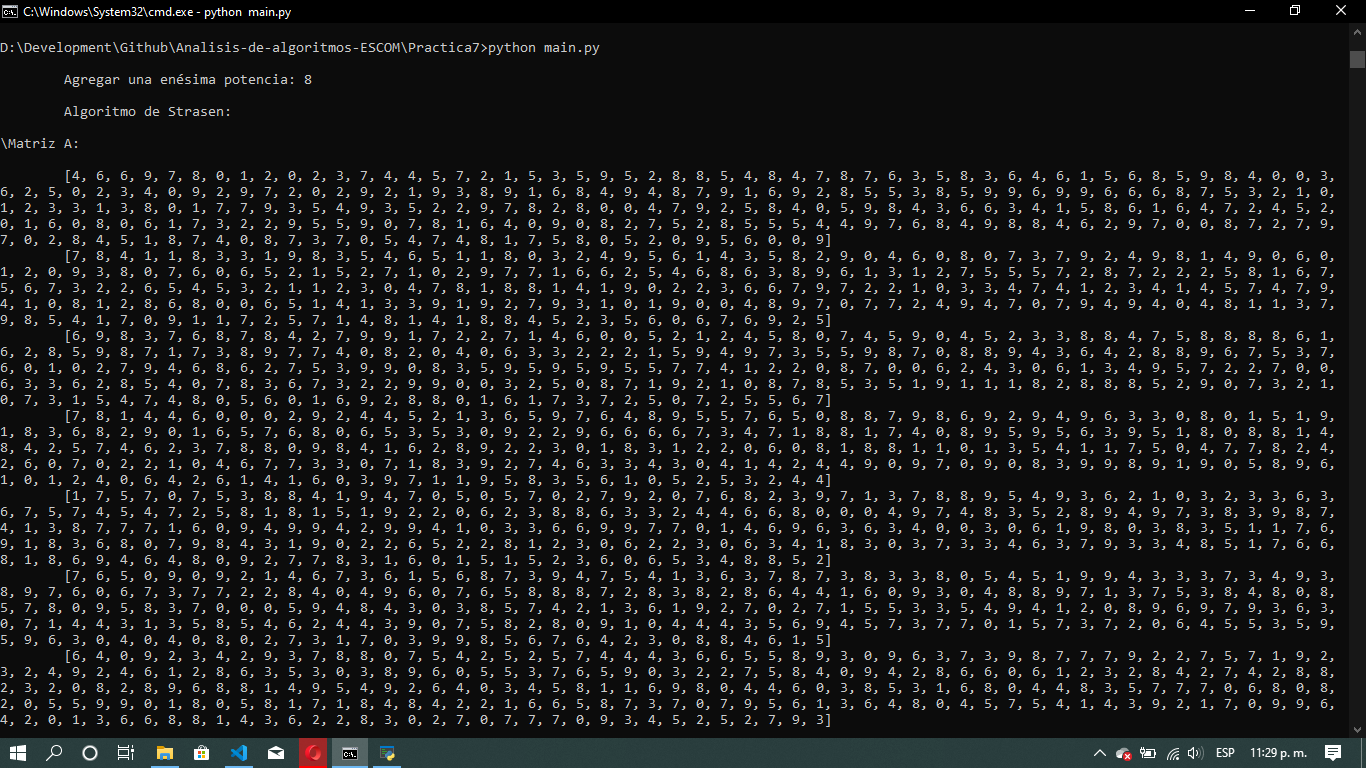
\includegraphics[scale=0.35]{vs1.png}
    \caption{Algoritmo de Strassen y producto cruz en ejecuci\'on}
    \label{fig:strassen_exec}
\end{figure}
\begin{figure}[H]
    \centering
    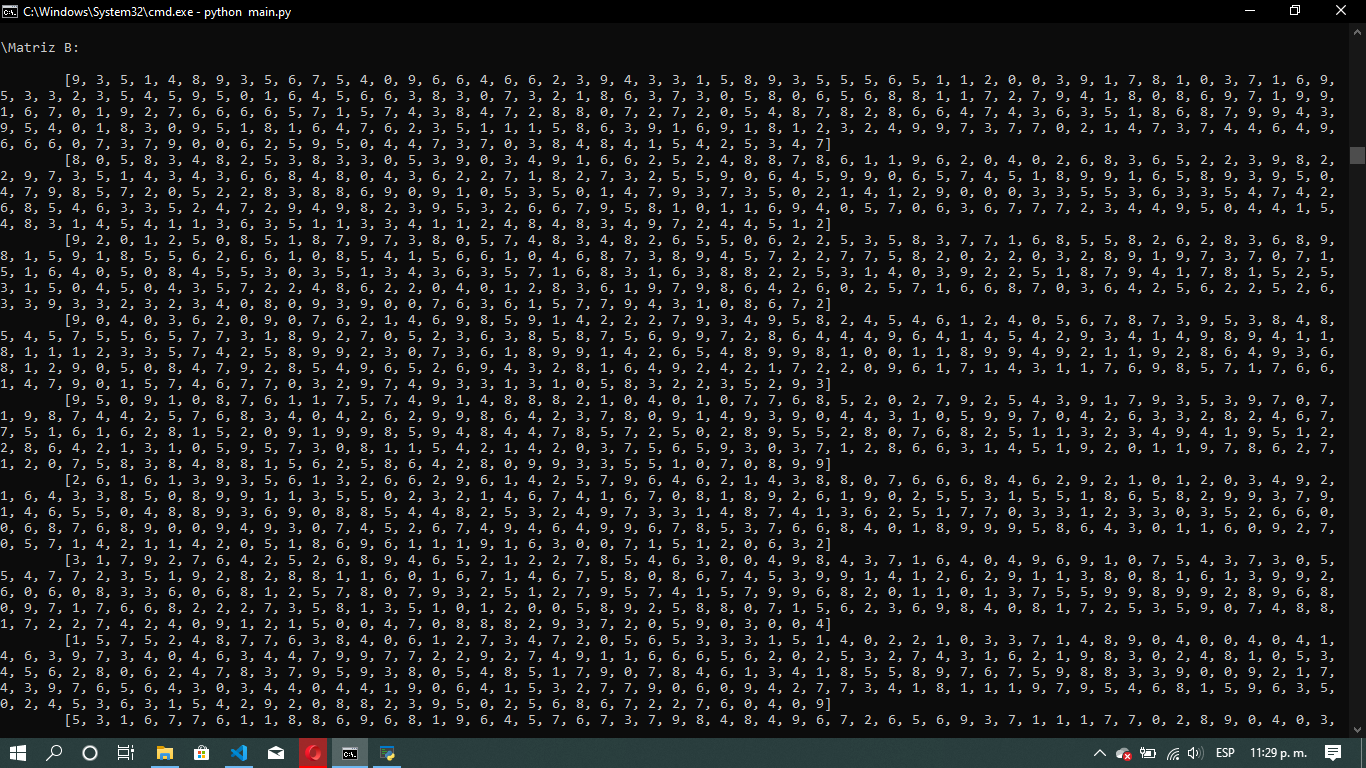
\includegraphics[scale=0.35]{vs2.png}
    \caption{Algoritmo de Strassen en ejecuci\'on}
    \label{fig:strassen_exec}
\end{figure}
\begin{figure}[H]
    \centering
    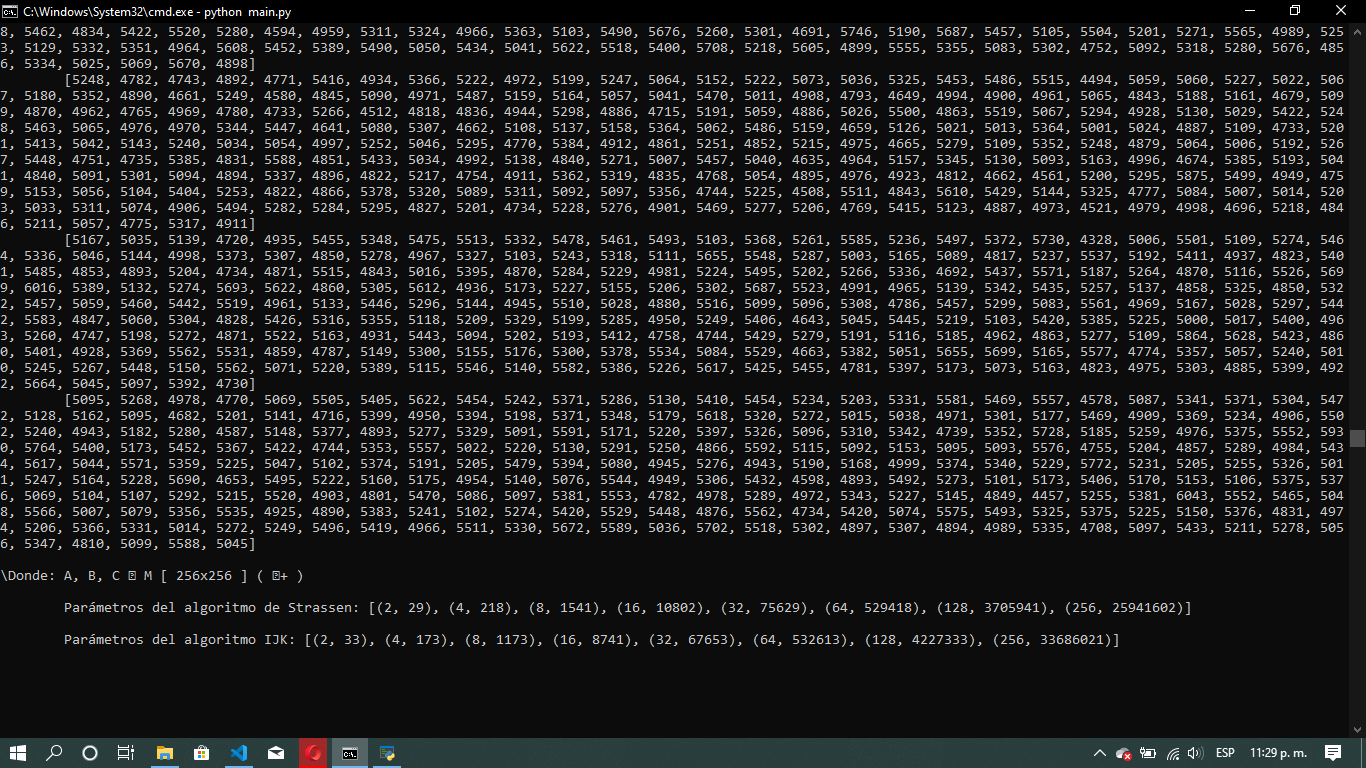
\includegraphics[scale=0.35]{vs3.png}
    \caption{Algoritmo de Strassen en ejecuci\'on}
    \label{fig:strassen_exec}
\end{figure}
\begin{figure}[H]
    \centering
    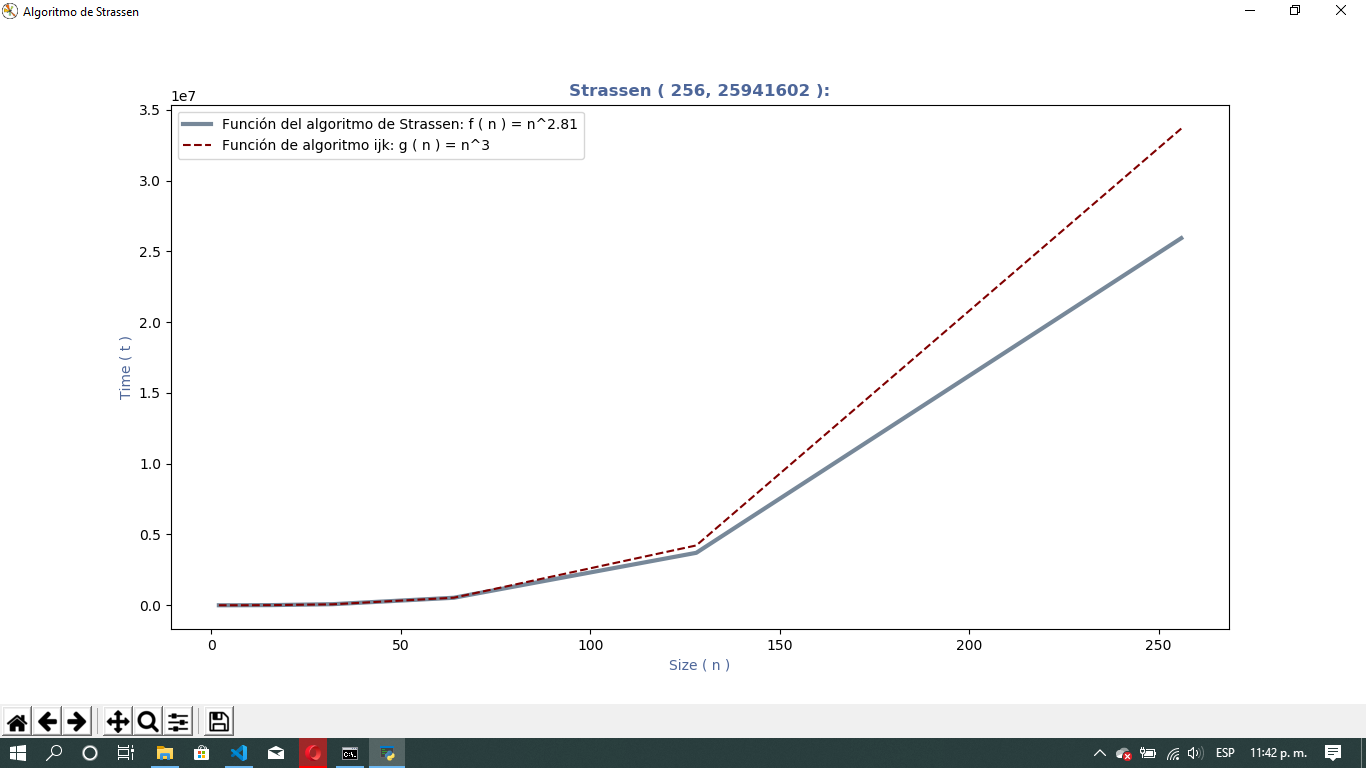
\includegraphics[scale=0.35]{vs4.png}
    \caption{Comparaci\'on del algoritmo de Strassen con el algoritmo usual, usando valores muy grandes}
    \label{fig:strassen_vs}
\end{figure}


\section{Conclusiones}

\textit{Alan Romero Lucero}. Este problema en particular me parece muy interesante, por el hecho de lo dif\'icil que es plantear un algoritmo que logre bajar su complejidad. Por ejemplo, con divide y vencer\'as me parece curioso que aplicando ese concepto no se pueda bajar la complejidad y quede igual que el algoritmo m\'as tradicional. Adem\'as, el algoritmo de Strassen es bastante peculiar, dadas la formulas que se tienen que permiten, aplicando muchas matem\'aticas, reducir la cantidad de multiplicaciones que se deben hacer por cuadrante de la matriz resultado. Su implementaci\'on es algo larga debido a la cantidad de operaciones que se tienen que hacer y la necesaria implementaci\'on de los algoritmos para sumar y restas matrices. Sin embargo, esta es una pr\'actica bastante interesante, y aun m\'as lo es este algoritmo que aunque no representa un gran avance en cuanto a complejidad, sirve como buen ejemplo.
\newline \newline
\textit{Josu\'e David Hern\'andez Ram\'irez}.
\newline \newline
El agoritmo de Strassen surgi\'o para hacer m\'as eficiente las operaciones con matrices, las cuales son usadas en varios aspectos que se usan hoy en d\'ia, como son la f\'isica de los motores gr\'aficos e inteligencia artificial, cuyo uso es obtener los resultados en el menor tiempo posible.
\newline \newline
Partimos de la complejidad del algoritmo 'usual' de multiplicaci\'on de algoritmos, la cual es $\theta(n^{3})$ y se refleja en en consumo de tiempo grande, y por ende, de recursos, la idea de optimizar la multiplicaci\'on de matrices ha persistido desde la creaci\'on del algoritmo presentado.
\newline
Como pudimos observar en la \'ultima figura, la complejidad unas decimas, el coste computacional reduce notablemente, haciendo m\'as f\'acil la implementaci\'on de estas operaciones.

\section{Bibliograf\'ia}
[1] GeeksforGeeks. (n.d.). Divide and Conquer | Set 5 (Strassen's Matrix Multiplication) - GeeksforGeeks. [online] Available at: https://www.geeksforgeeks.org/strassens-matrix-multiplication/ [Accessed 14 Oct. 2019].

\end{document}